\chapter{Spin Analysis}
\section{Classification of Signal or Background Events}
After producing our data set, engineering features which help us convert our
experimental data into observables, we are then tasked with the problem of
separating out signal events from background events. Many processes are capable
of producing muons, many of which are dominant in the $W$ boson kinematic
regime (Figure~\ref{fig:muon_production_vs_pt}).

\begin{figure}[H]
	\begin{center}
		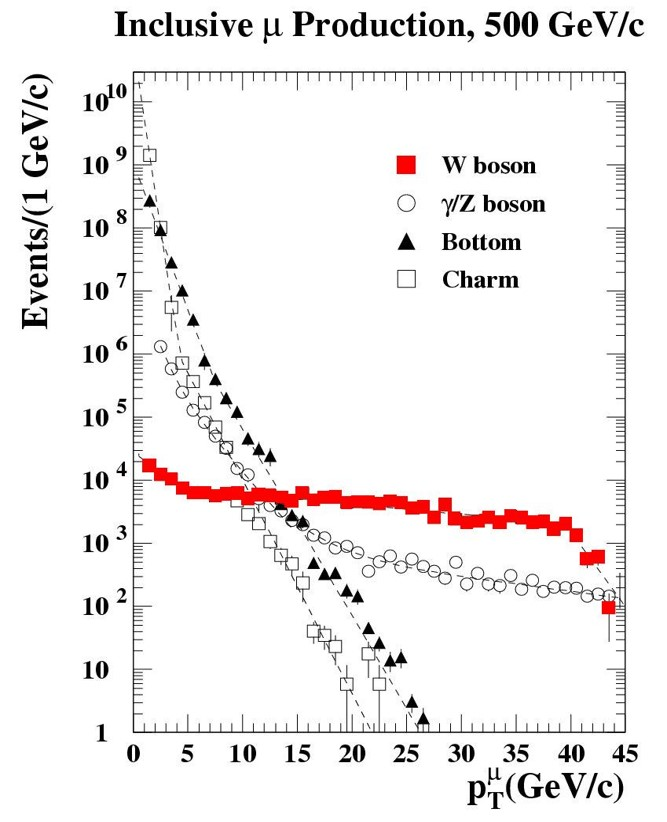
\includegraphics[width=0.5\linewidth]{./figures/muon_production_vs_pt.jpg}
		\caption{ Observing the simulated production of muon as a function of $p_T$, we
			can see that in the kinematic region of $W$ production that the dominant sources
			of muons come from other processes. The new PHENIX muon trigger threshold is
			sensitive at 10 $GeV/c$ and above. }
		\label{fig:muon_production_vs_pt}
	\end{center}
\end{figure}

We can divide up the total observed muon spectrum into contributions from three
sources:

\begin{itemize}
	\item Real Muon Background
		\begin{itemize}
			\item Z,$\gamma^*$
			\item $W\rightarrow$had
			\item $W\rightarrow$tau
		  \item onium
			\item open charm
			\item direct photon
		\end{itemize}
	\item Fake Muons (Hadronic Background)
		\begin{itemize}	
			\item Hadrons which are reconstructed as high $p_T$ muons due to detector
			resolution.
		\end{itemize}
	\item Signal Muons
		\begin{itemize}	
			\item Real $W\rightarrow\mu$ events.
		\end{itemize}
\end{itemize}

Previous analyses have attempted to separate the muon spectrum into $p_T$ bins,
to estimate the composition, however, because the $W\rightarrow\mu$ signal is so
small in the forward kinematic regime, these methods are not sufficient, as
there is no 'visible' cutoff in the spectrum. However, by using simulations.
However, we may use other methods to split up our spectrum, with the ultimate
goal of calculating $A_L$, and correcting for background dilution using the
signal to background ratio. We must use another method to effectively describe
the difference between an event which comes from a signal, vs background event.

\subsection{Naive Bayes Classification}
There are many techniques available for classifying a collection of variables
(a feature set) into categories. Naive Bayes classification is an excellent
candidate for classification, in cases where we have two classifications with
distributions of featuresets which are uncorrelated. Naive Bayes even works when
feature sets are slightly correlated. It is a robust, fast, scalable machine
learning technique. Traditionally used for classification of text documents,
Naive Bayes is also able to handle numeric features whose distributions are
known \cite{Collins2013}.

In our analysis, we begin with a Naive Bayes classifer which is trained to
classify two signal muons, vs background muons. We combine both Real Muon
Background muons and Fake Muons (Hadronic Background Muons) in the label of
"Background Muons" at this stage, though, later, we will separate out the muons
further.

The descriniating variables described in~\ref{ch:data_collection} were
chosen from the multitude of possible physical event parameters, because they
were all maximally uncorrelated. Concretely, these correlations are presented in

\begin{figure}[H]
	\centering
	\begin{subfigure}{0.5\textwidth}
		\centering
		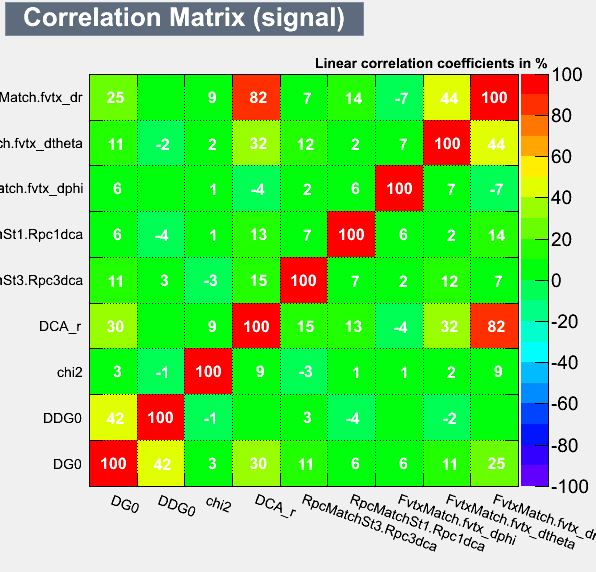
\includegraphics[width=0.95\linewidth]{./figures/CorrelationMatrix_Signal.png}
		\caption{Correlations between kinematic variables, produced from simulated
			data.}
		\label{fig:corr_mat_sig}
	\end{subfigure}%
	\begin{subfigure}{0.5\textwidth}
		\centering
		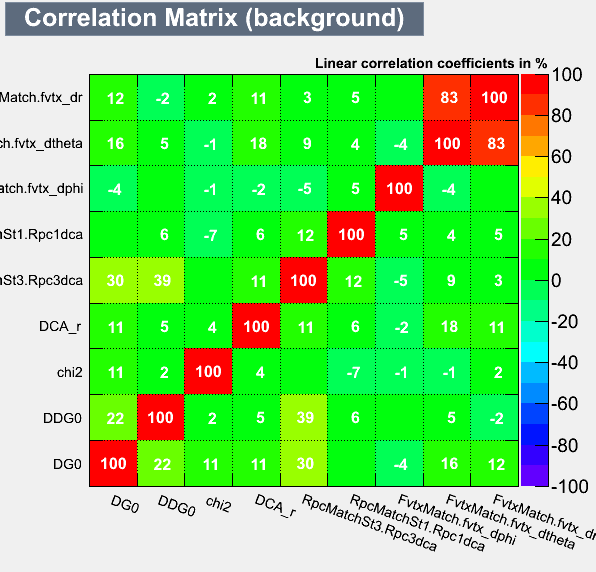
\includegraphics[width=0.95\linewidth]{./figures/CorrelationMatrix_Background.png}
		\caption{Correlations betwen kinematic variables, produced from the data,
			which is composed mostly of hadronic background}
		\label{fig:corr_mat_bkg}
	\end{subfigure}
	\caption{ Low correlations between the signal variable distributions (from
		simulation), and the background variable distributions make this data set a
		good candidate for classfication using Naive Bayes}
	\label{fig:kinematic_var_correlations}
\end{figure}

Briefly, a Naive Bayes classifier may be constructed from the core of the
familiar Bayes Theorem from probability and statistics.

In our case, we understand Naive Bayes as a conditional probability. Concretely,
we consider a vector of features (i.e. our discriminating kinematic variables):
\begin{equation}
	\label{eq:feature_vector}
\mathbf{x} = (x_1, \dots, x_n)
\end{equation}

and assume independence between each feature $x_n$. We then define the
probability of a given classification, $C_k$ given a set of features $x_n$:

\begin{equation}
	\label{eq:cond_probabilty}
p(C_k \vert x_1, \dots, x_n)
\end{equation}

This conditional probability is defined in terms of Bayes Theorem:

\begin{equation}
	\label{eq:bayes_theorm}
p(C_k \vert \mathbf{x}) = \frac{p(C_k) \ p(\mathbf{x} \vert C_k)}{p(\mathbf{x})}
\end{equation}

The terms here are defined as:
\begin{itemize}
	\item $p(C_k)\rightarrow$ prior probability
	\item $p(\mathbf{x} \vert C_k)\rightarrow$ likelihood
	\item $p(\mathbf{x})\rightarrow$ evidence
\end{itemize}

In principal, the final step in a classifier is to assign a class. This is done
by computing the probability of a feature-set belonging to one class, or to
another class, using Bayes Theroem. The class with the larger proability is than
taken as the defacto classification of that particular feature set. However, we
may instead observe these probabilities directly, and label data with this
probability. This is what we ultimately call our "$W_{ness}$" parameter. This
will be discussed in section~\ref{ssec:likelihood}.

\subsection{Composition of Probability Distribution Functions}
After we have engineered appropriate features to use in the analysis, we can
proceed with composing probability density functions so we can proceed with the
calculation of likelihoods, which will label our data set, allowing us to reduce
our data set further from the basic cuts, without removing any signal events.


\subsection{Labeling Data With Likliehood Ratio: $W_{ness}$}
\label{ssec:likelihood}
\section{Extended Unbinned Maximum Likelihood Fits}
\subsection{Modeling The Hadronic Background}
\subsection{Modeling the Muon Background}
\subsection{Modeling the W-Signal}
\subsection{Overview}
\subsection{Fit Performance}
\subsection{S/BG and Muon Backgrounds}
\label{ssec:sbr}
\subsection{$W_{ness}$ Dependence of S/BG}
\section{Calculation of $A_{L}$ for $W\rightarrow\mu$}
\subsection{Overview}
\subsection{Asymmetry Calculation}
\subsection{Discussion of Work Done By Analysis Team}
\section{Data Validation}
Mention Daniel's GPR, Ralf's PEPSI, Abraham's FVTX work, and Francesca's cross-checks.
\subsection{Simulations and The Signal to Background Ratio}
\subsection{Gaussian Process Regression}
\subsection{Four Way Cross Validation}
\subsection{Asymmetry Consistency Check}
\subsection{Beam Polarization}
\subsection{Beam Luminosity}
\subsection{Code Cross Validation}
